\clearpage%if the chapter heading starts close to bottom of the page, force a line break and remove the vertical vspace
\vspace{21.5pt}
\chapter{Implementation}\label{ch:proposed-solution}

The following sections detail the implemented solution to flag network traffic as malicious or benign.
The criteria for selecting tools used in the implementation was that they be freely available and open-source.
The implemented solution was divided into two separate parts, namely the network environment setup and model training parts.

The network environment setup dealt with generating malicious and benign traffic in a virtualized environment to be used later in testing the prediction of the models trained.
This part was not strictly necessary as traffic can be generated and captured in any network environment;
the rationale of creating such an environment was to capture only needed traffic in a safe environment, to keep the size of
capture packets small, and to increase privacy as captured packets might contain other network data when capturing in \gls{pr-mode}.

The model training part was concerned with creating machine learning models to analyze and flag the captured traffic in the virtual network.
Additionally, it also dealt with choosing the dataset used in training the models and other details involved in the whole process.


\section{Network Environment Setup}\label{sec:environment-setup}
The virtualized network environment was created with the help of \emph{Vagrant};
\emph{Vagrant} is a tool that can be used to quickly provision virtual machines.
The environment created with \emph{Vagrant} consisted of three machines all in the same network for simplicity since the aim was to generate and capture traffic.
All machines were created using a base image of Kali Linux, which is a popular OS used commonly in security testing scenarios.
The names and roles were assigned were as follows:

\begin{itemize}
    \item \emph{defender}: to capture traffic in the network
    \item \emph{attacker}: to generate malicious traffic
    \item \emph{target}: to act as a vulnerable server that can be attacked.
\end{itemize}

The \emph{target} machine had a version of \gls{dvwa} running on it.
\gls{dvwa} is an intentionally insecure web application which makes it a good candidate for testing malicious attacks.
The vulnerabilities discussed in chapter ~\ref{sec:malicious-network-traffic} are all possible in \gls{dvwa}.

\begin{code}
    \begin{minted}{ruby}
  config.vm.define "vulnerable-target" do |target|
    target.vm.hostname = "target"
    target.vm.network "private_network", ip: "192.168.60.60"
    target.vm.provider :virtualbox do |vb|
      vb.gui = false
      vb.name = "target"
      vb.memory = 1024
      vb.cpus = 1
    end
    target.vm.provision "bootstrap", type: "shell", path: "./make_dvwa_accessible_to_lan.sh", run: "once"
    target.vm.provision "start-dvwa", type: "shell", inline: "sudo dvwa-start", run: "always"
  end
    \end{minted}
\captionof{listing}{Provisioning the \emph{target} machine with \emph{Vagrant}}
\label{code:vagrant-target-provision}
\end{code}

The listing \ref{code:vagrant-target-provision} shows the code used in creating the \emph{target} machine.
While it is possible to use other providers, \emph{Virtualbox} was chosen because it had support in \emph{Vagrant} to modify
network device settings which was needed to set \gls{pr-mode} in the \emph{defender} machine.


With the virtual \gls{lan} created, the network traffic was generated in both malicious and benign stages.
In the malicious stage, the \emph{attacker} generated traffic for \gls{DoS}, \gls{sql} injection, command injection, brute force, and \gls{xss} attacks.
The \emph{attacker} machine in figure \ref{fig:attacker-box} shows how malicious network traffic was generated in the case of \gls{sql} injection that was aimed at the \emph{target} machine.

\begin{figure}[H]
    \centering
    \AltText{A view of the attacker machine OS interface showing a terminal client in the left-hand side and a web browser in the right-hand side}{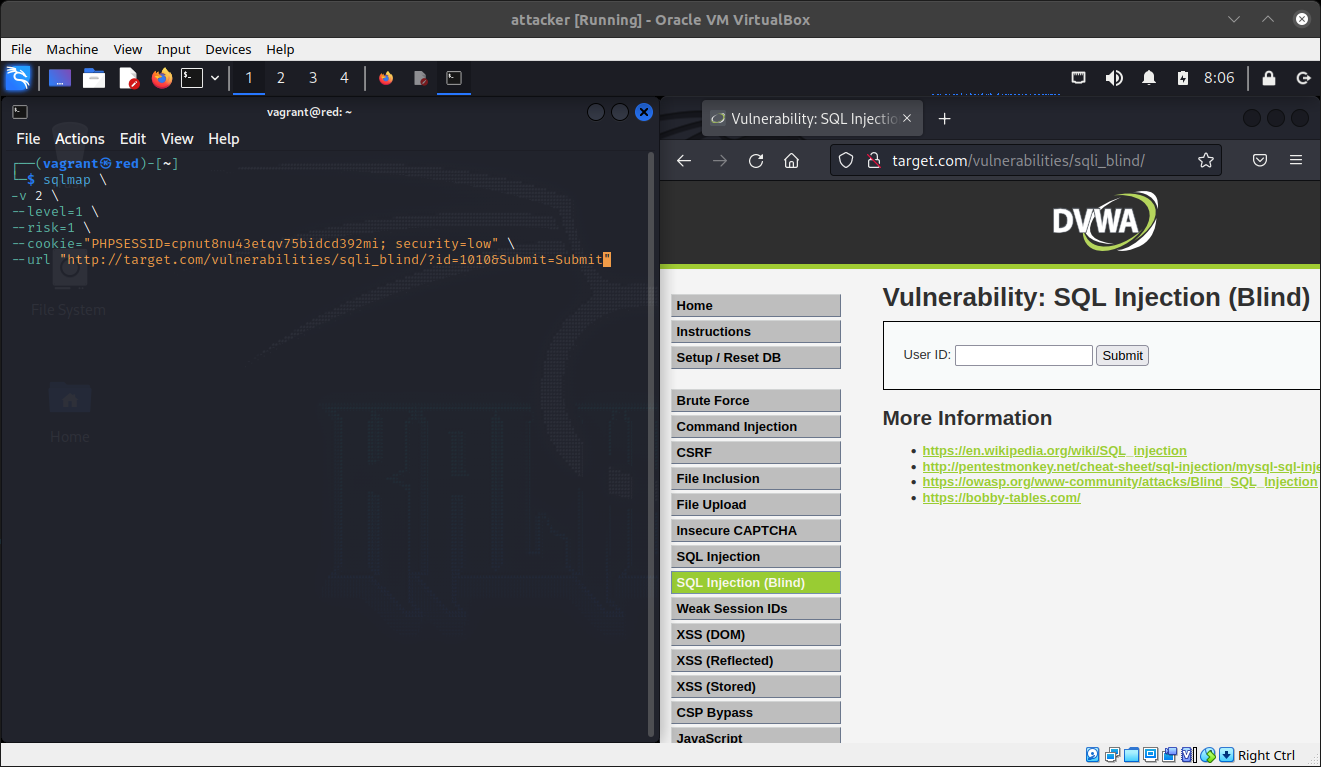
\includegraphics[width=\textwidth]{attacker-view}}
    \caption{Screenshot of \emph{attacker} machine preparing an \gls{sql} injection test}
    \label{fig:attacker-box}
\end{figure}


The figure \ref{fig:attacker-box} shows in view the web application to be attacked and the program \emph{sqlmap} to automate discovery of \gls{sql} vulnerabilities.
In contrast to the malicious stage which consisted only of traffic captured in the virtual \gls{lan},
the benign stage consisted of both virtual \gls{lan} and internet directed traffic.
The benign traffic consisted of web browsing of the \emph{target} machine's web application via \gls{http} without any attacks.
The rest of the benign traffic consisted of Telnet, \gls{dns}, \gls{ssh}, and \gls{ftp} protocol-related traffic.
Each scenario of the malicious and benign stages was captured in \gls{pcap} file format by the \emph{defender} machine using \emph{tcpdump}.
As a final step, the benign \gls{pcap} files were renamed to include the word `benign' in the filename to distinguish them from the malicious captures.


\section{Model Training}\label{sec:model-training}

This section focuses on the model training process and how it was implemented with machine learning methods:
\gls{knn}, Logistic Regression, \gls{mlp}, and Random Forest.
Training the models involved feeding them with labeled data to learn the patterns and relationships within the data.
The training was performed on a laptop with an `AMD® Ryzen 7 PRO 4750U' processor and 30.6 GiB of SODIMM DDR4 memory.

\subsection{Dataset}
The training process for classification tasks needs labeled data for supervised machine learning.
The quality, quantity, and representativeness of the dataset used can greatly impact the performance of the trained models.
It was deemed that the labeled data should contain at least some features that can be extracted (\gls{feat-extr}) easily from \gls{pcap} files.


The dataset eventually selected for use was the CICIDS2017 intrusion detection evaluation dataset \cite{sharafaldin2018toward}.
A newer version did exist at the start of the implementation (CSE-CIC-IDS2018), nonetheless CICIDS2017 was used due to its relative small size (under 900 MB).
The CICIDS2017 dataset with labeled data existed in CSV file format, those were downloaded and used in the model training.
Figure \ref{fig:dataset-label-dist} visually shows the composition of the CICIDS2017 dataset.

\begin{figure}[ht]
    \centering
    \AltText{A bar plot showing the distribution of labels in dataset with y-axis showing label count in logarithmic scale and x-axis showing the name of the attack label}{\includesvg[width=\textwidth]{dataset_label_distribution}}
    \caption{Dataset label distribution}
    \label{fig:dataset-label-dist}
\end{figure}

\clearpage
The dataset label distribution can be observed in figure \ref{fig:dataset-label-dist} showing the proportion of malicious labels to benign labels.
Due to the proportion of benign labels being higher in comparison to malicious labels (2,271,320 versus 556,556), one CSV file from the dataset (\texttt{\detokenize{Monday-WorkingHours.pcap_ISCX.csv}}) was dropped from the training process since it contained only benign labels.
The dataset was further preprocessed by removing identified redundant columns and one duplicate column;
moreover rows with infinity numbers were removed the dataset.
Finally, the columns with malicious labels were converted to the class number one while
benign labels were converted to the class number zero to make the training process straight-forward.
In the end the combined dataset after preprocessing had 2,298,395 rows with 71 columns where seventy columns were for features and one column for labels.


\subsection{Training Process}
The model training part as stated previously involves finding patterns within the dataset to make predictions for whether a particular piece of network traffic is malicious.
In the implementation of this stage, the \emph{scikit-learn} \cite{scikit-learn} library was chosen due to the availability of documentation and examples;
another reason was that it did not have any dependencies to GPU libraries, making it easy to install on different OS platforms.
The use of a machine learning library significantly reduced the implementation time since no time would be spent on algorithm coding.
The steps involved in the training process consisted of:

\begin{itemize}
    \item Creating the model pipeline.
    \item Training and tuning of \gls{hyper-param}.
    \item Cross-validation of models.
    \item Saving models in a persistent format.
\end{itemize}

The model pipeline is a list of steps that are chained together and can be applied to a piece of data input.
Listing \ref{code:knn-pipe} shows a \gls{knn} model pipeline as used in the training process implementation.
\clearpage

\begin{code}
    \begin{minted}{python}
def knn_model() -> Pipeline:
    return make_pipeline(
        StandardScaler(),
        LinearDiscriminantAnalysis(),
        KNeighborsClassifier(
            n_neighbors=3,
            p=2,
        ),
        verbose=True,
    )
    \end{minted}
\captionof{listing}{Setup of \gls{knn} pipeline}
\label{code:knn-pipe}
\end{code}

The pipeline shown in listing \ref{code:knn-pipe} contains three steps: scaling, dimensionality reduction, and the K-neighbors classifier itself.
The scaling of features step is an additional preprocessing step which depending on the learning algorithm itself might be needed or not;
in addition, the dimensionality reduction step helps reduce computation time---here it reduces the data dimensions from 70 to 1.
The last step in the pipeline is the \gls{knn} classifier with $K=3$ and $p=2$ to use the Euclidean distance metric (see chapter \ref{knn:theory}).
Contrast the parameters in listing \ref{code:knn-pipe} with listing \ref{code:rf-pipe}.

\begin{code}
\begin{minted}{python}
    return make_pipeline(
        RandomForestClassifier(
            n_estimators=100,
            criterion="gini",
            max_depth=None,
            max_features=35,
            min_samples_split=2,
            min_samples_leaf=2,
            bootstrap=False,
            max_samples=None,
            random_state=SEED,
            verbose=1,
            class_weight="balanced",
        ),
        verbose=True,
    )
\end{minted}
\captionof{listing}{Setup of Random Forest pipeline}
\label{code:rf-pipe}
\end{code}

\clearpage
As can be noted in listing \ref{code:rf-pipe}, some models can have more tunable \gls{hyper-param}.
Another difference that can be observed is that Random Forest does not need feature scaling since the algorithm is not sensitive to unscaled features.
Furthermore, the pipeline contains only one step so essentially the classifier can be used directly without including it in a pipeline;
the reason it was included is to make it easily comparable to the other models and additionally for code type checking.

The training part is straight-forward, the dataset is split into \gls{train-data} and \gls{test-data},
the portion of the \gls{test-data} was chosen to be a third of the dataset.
Each time the model pipeline was ran, the test score (calculated on the \gls{test-data}) and time taken was noted.
By tuning the \gls{hyper-param}, varying test scores could be observed;
in this way, a specific model's \gls{hyper-param} that perform best were eventually used.
Note that, the \gls{hyper-param} that had good performance where not necessarily used in the final training,
the time to train the model was also taken into account.
Therefore a balance between the two was the deciding factor on which \gls{hyper-param} were used.
For training the final models with the parameters chosen---the whole dataset is used, there was no need to set aside \gls{train-data}.

Be aware that there exist software libraries to automate the tuning of \gls{hyper-param} to find the best performing parameters or even the best predictive model itself.
This path was abandoned after a few rounds due to unreliability problems where the process would crash after a few days of training.

Additionally, \gls{cv} of the models was performed.
This was done to ensure that the models were not \gls{over-fitting} on the \gls{train-data}.
The \gls{cv} strategy chosen was a stratified k-fold wherein the \gls{train-data} was split into five folds and
the test score accuracy was compared.
A stratified strategy in the \gls{cv} was crucial since the dataset labels were not in equal proportions (see figure \ref{fig:dataset-label-dist}).

\clearpage
The last step in the training process was saving the models trained.
The importance of this step is that there is no need to train the model again in order to use it in network traffic prediction---this saves time and computation resources.
The other rationale is if sharing of the model is needed later.
There exist several formats for saving models, each with their advantage and disadvantages, for this implementation, the \emph{skops} library was chosen.
The main reason \emph{skops} was chosen is that it was created to work with the \emph{scikit-learn} library which made it easy to integrate within the project.
One disadvantage however with \emph{skops} is that the models trained cannot be imported in other programming languages,
therefore the saved models can only work with the specific version of Python programming language and \emph{scikit-learn} library used in the training process.

\subsection{Prediction Process}
Before the prediction based on the saved models was done, the \gls{pcap} files were first converted to CSV files;
this was done with the help of a software project called \emph{cicflowmeter}.
The version available at the time the project started was forked and modified to fix some errors and consequently included in this project
to do the conversion part.
The importance of the conversion from \gls{pcap} to CSV is that \gls{feat-extr} is performed on the network traffic data.
The \gls{feat-extr} process itself is out of scope of this thesis.
However, it suffices to say that \emph{cicflowmeter} (Python implementation) is based on \emph{CICFlowMeter} which is a Java software associated with the CICIDS2017 dataset used for feature extraction, among its other uses.


The prediction process in the implementation consisted of predicting the collected network traffic from the \gls{lan}.
For quick predictions, a \gls{gui} was created to facilitate this process as show in figure \ref{fig:gui}.


\begin{figure}[H]
\centering
\AltText{A GUI that shows three buttons, one for selecting the model, second for selecting the PCAP file and the third for predicting whether it is malicious or benign}{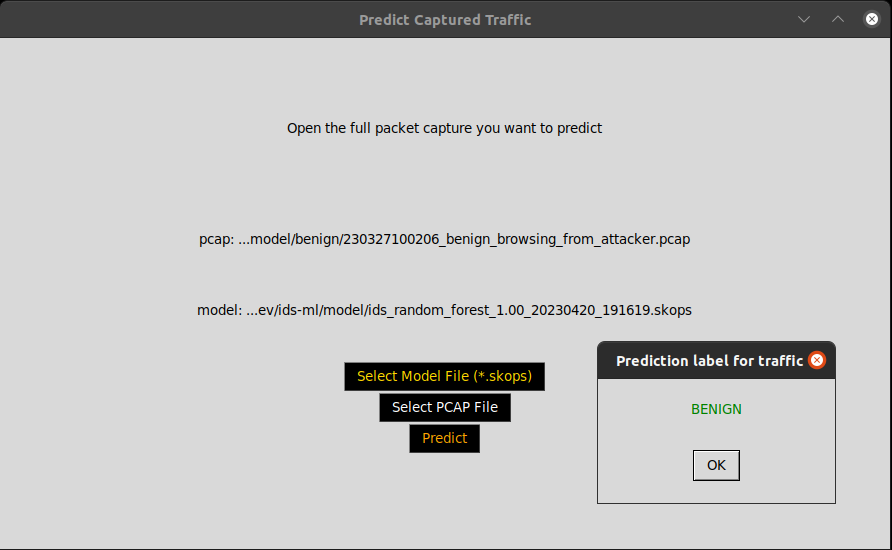
\includegraphics[width=\textwidth]{gui}}
\caption{Screenshot of the simple prediction \gls{gui}}
\label{fig:gui}
\end{figure}

The \gls{gui} in figure \ref{fig:gui} was created through Python's interface to the Tcl/Tk \gls{gui} toolkit called \emph{tkinter}.
The choice for using \emph{tkinter} instead of other more newer \gls{gui} toolkits, for instance, the \emph{Qt} framework, was
simply because the functionality desired was basic, namely, a few buttons, and a way to open files.

Through testing prediction of different models over time, it became cumbersome to observe and record predictions in this way.
As an alternative, a script to run predictions of different models on multiple \gls{pcap} files was implemented;
the script was meant to create a simple report showing how correct the predictions were in reality.
Figure \ref{fig:t-report} shows how the report looked in practice.


\begin{figure}[H]
\centering
\AltText{A text file showing the predictions for two models. It also show a summary of how many predictions were true and false}{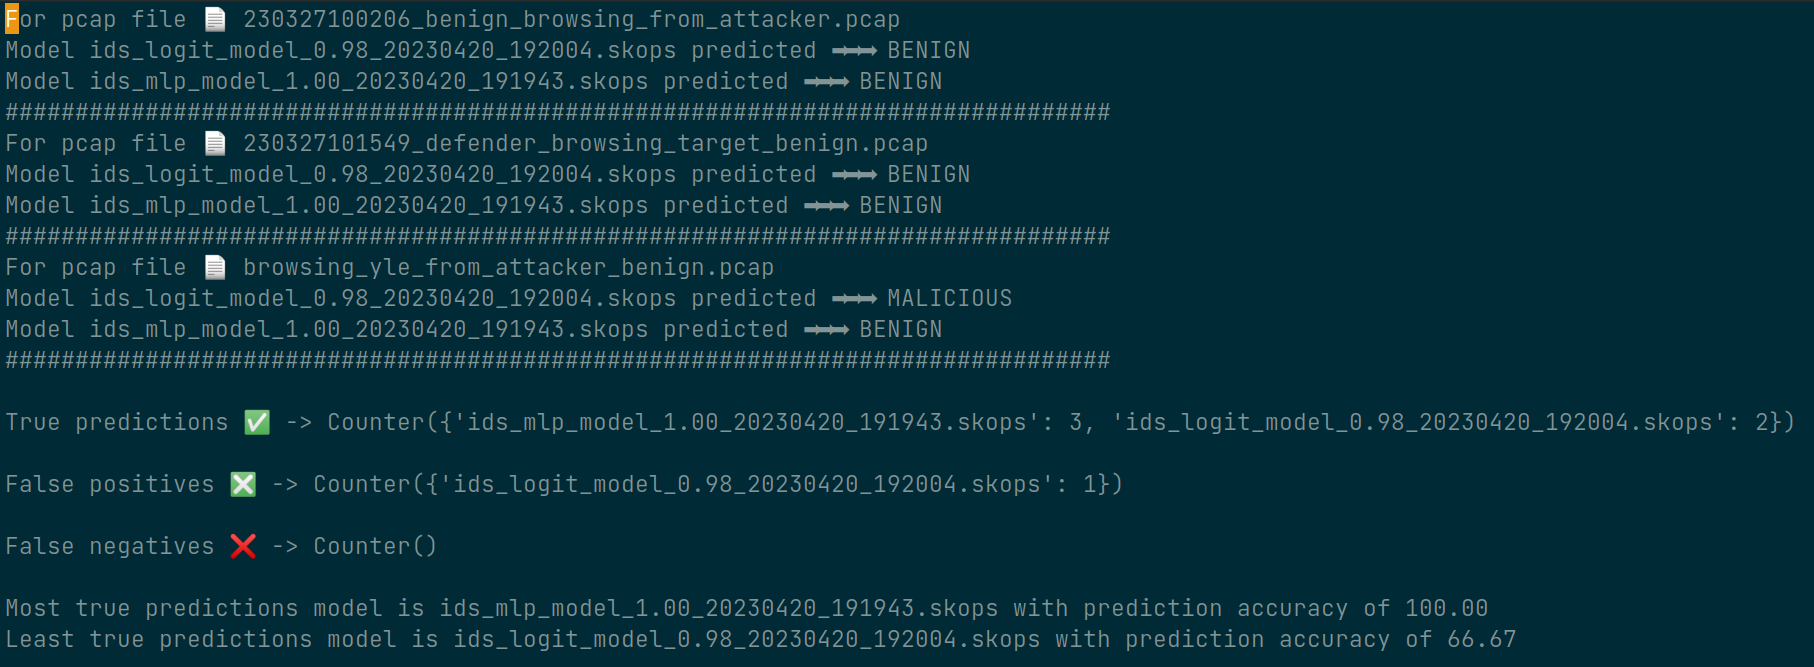
\includegraphics[width=\textwidth]{comparison-report}}
\caption{Screenshot of the simple report content}
\label{fig:t-report}
\end{figure}

The figure \ref{fig:t-report} also shows that the simple report created by the script details the count of true predictions, \gls{false-positive}s and \gls{false-negative}s.
Both the \gls{gui} and the script methods were used in different scenarios depending on what effort was required in regards to whether a single prediction was desired or multiple.

The full source code for the solution implementation can be found at \href{https://github.com/nicolaskyejo/ids-ml-exploration}{https://github.com/nicolaskyejo/ids-ml-exploration},
it contains both the network environment setup and the model \gls{hyper-param} used for the results obtained in the following chapter.
